
\chapter{Maximal torque capacities}
\label{chapter:maximaltorquecapacities}
\section{Introduction}

In the upper-limb, maximal torque capacities denotes the feasible \textit{3D strength} of each joint, represented as a set.
In isometric conditions, it should reflect multiple biomechanical properties observed experimentally, such as:
it depends on the muscle geometry ([REFS]), on the considered posture ([REFS]), 
on the muscle maximal tensions ([REFS]), the muscle volumes ([REFS]), the muscle tension interactions ([REFS]) but also 
anthropometric considerations like the age ([REFS]), the bones structure ([REFS]), and also the physical fatigue ([REFS])
and the cognitive charge ([REFS]).

Consider a musculoskeletal model $\mathcal{M}$ described as a kinematic chain of $n$ degrees-of-freedoms (DOF)
and $m$ muscles. Every muscle produce a . All muscle tensions can be summarized in a matrix $L\in \mathbb{R}^{m\times n}$
called the \textit{lever arm} matrix:

$$L = \left(\frac{\partial l_i(\mathbf{q})}{\partial \mathbf{q}}\right)_{i=1,\dots,m}$$

By denoting $t_i(\mathbf{q})$ the tension exerted by muscle $i$, it is possible to describe the projection of 
the muscle tensions onto the joint torque space:
$$\tau = -L^T\mathbf{t}$$


\section{Representation in musculoskeletal models with a small number of muscles}
\subsection{Zonotope representation}
\begin{definition}
    A \textit{zonotope} is the projection of a cube.
\end{definition}


\begin{figure}[h]
    \centering
    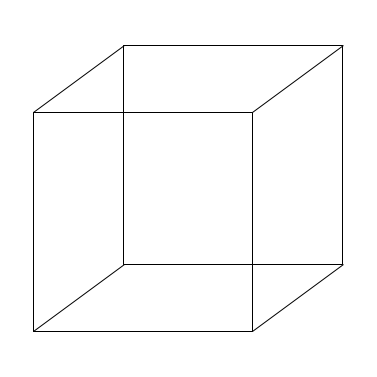
\includegraphics[width=0.3\linewidth]{img/zonotopes/Cube3D.png}
    \caption[A $3$-cube]{A $3$-cube}
    \label{im:3Dcube}
\end{figure}

The concept of a zonotope is well-known and was primarly studied in crystallography.
Zonotopes are a particular subject of matter due to the parallelness of their faces, which
interest crystallographers.

Consider now that muscle tensions are bounded, \textit{i.e.} for each muscle $i$ and every joint configuration $\mathbf{q}$,
there exist $\underline{t_i}(\mathbf{q}), \overline{t_i}(\mathbf{q}) \in \mathbb{R}$ such
that $0 \leq \underline{t_i}(\mathbf{q}) \leq t_i(\mathbf{q}) \leq \overline{t_i}(\mathbf{q})$.

This chapter will assume that all muscles apply their tension independently from another muscle, so that 
all possible tension combinations are described by an $m$-\textit{orthotope}, which is the geometric name for 
denoting a hyperrectangle of dimension $m$.

Any feasible tension combination is thus $\mathbf{t}(\mathbf{q}) \in \mathcal{O}(\mathbf{q}) := 
\left[\underline{t_1}(\mathbf{q}),\, \overline{t_1}(\mathbf{q})\right] \times
\dots \times
\left[\underline{t_m}(\mathbf{q}),\, \overline{t_m}(\mathbf{q})\right] $

In this case, we have for a specific joint configuraiton 
$\tau = -L^t\mathbf{t}$ for $\mathbf{t}\in\mathcal{O}$. Since $\mathcal{O}$ is a convex set, 
then $\tau$ can be described as a convex set as well (affine transformation of a convex set).
This set is denoted $\mathcal{Z}_{\tau}$ and this is the torque zonotope:
$$\mathcal{Z}_{\tau} = \left\{-L^T\mathbf{t} \mid \mathbf{t}\in \mathcal{O} \right\} = -L^T\mathcal{O}$$

It is simple to show that $\mathcal{Z}_{\tau}$ is indeed a zonotope: while a zonotope has been defined as a 
projection of a $m$-cube, notice that a $m$-orthotope is a affine invertible transformation of a $m$-cube
consisting of an invertible anisotropic dilation and a translation. In other word, $\mathcal{O} = D\mathcal{C} + T$,
with $D$ a strictly positive diagonal matrix. 

\subsection{Computing vertices and hyperplanes of zonotopes}
While zonotopes are compactly written through generators, this affine projection do not gives sufficient information
on its surface $\partial \mathcal{Z}$. It only describe how the zonotope is structured.
There is a huge interest in computing the vertices or an hyperplane description of a zonotope: in [REF], hyperplanes
are used for detecting collision.


\subsection{Edges and vertices enumeration algorithm}
For $n\leq m \in\mathbb{N}$, consider a $n$-zonotope $\mathcal{Z} = N\mathcal{C}$, 
with $\mathcal{C}$ a $m$-cube and $N\in \mathbb{R}^{n\times m}$ an affine map of rank $n$.

\textit{Enumerating} vertices of a zonotope is the process 
of listing all its vertices on its surface. Most enumeration algorithms use the computation of the \textit{convex hull} of 
a set, which is the smallest convex set containing it. For a set $S$, it is usually noted $\text{hull}(S)$ or $\text{conv}(S)$.
This operation is well-defined and suitable for computation when using a set of points. One of the most 
suitable algorithm for $k$ points in dimension $d > 3$ is \textit{Quickhull} \cite{barberQuickhullAlgorithmConvex1996}, which has an expected time complexity 
of $O(k\log k)$ ($O(k^2)$ in the worst case). 

\begin{figure}[h]
    \centering
    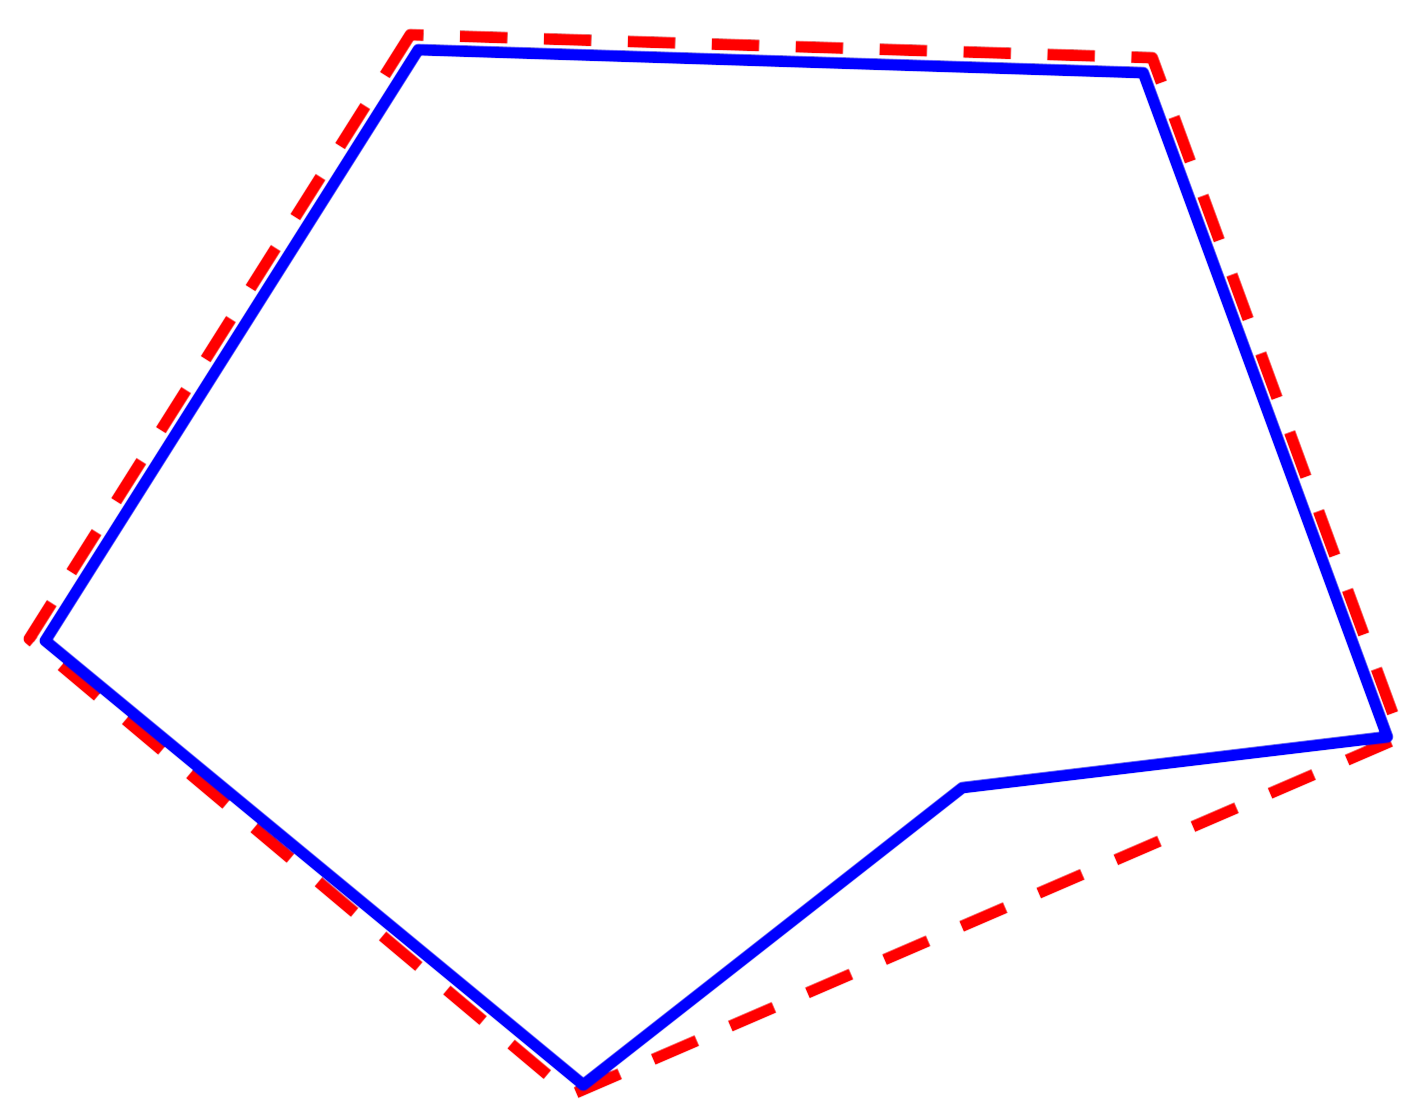
\includegraphics[width=0.4\linewidth]{img/zonotopes/convexHullExample.png}
    \caption{In blue: a non-convex polygon; in dotted red: its convex hull.}
    \label{im:convexHull}
\end{figure}


To enumerate the vertices of $\mathcal{Z}$, a naive algorithm would require to enumerate 
all of the $m$-cube vertices, project them via $N$ and compute the convex hull of all these points.
Unfortunately, the number of vertices of a $m$-cube is $2^m$ so that the expected complexity of the convex hull 
will reflect it.

While there are algorithms to compute vertices or hyperplanes of a zonotope such as the \textit{reverse search algorithm} 
(Fukuda, 1996) or the hyperplane shifting method (HSM) (Gouttefarde and Krut, 2010), 
none of them use one major property of zonotopes:
its edges are parallel to one of its generators. At first, it may seem unreasonnable to enumerate edges,
because there are $m\times 2^{m-1}$ edges in a $m$-cube, which is \textit{much} more than the number of 
its vertices when $m$ is large: for 
instance, a $10$-cube consists of $1024$ vertices and $5120$ edges.

However, 

\subsubsection{Convex hull of parallel lines}

However, the convex hull of a set of lines is a much harder problem. 
We suggest here a straight-forward algorithm 
to compute it in the case where all lines are parallel. The main idea is that since all lines are parallel, only 
their translation from the origin distinguish them; this translation information being described as a vector,
it is possible to reduce the convex hull of parallel lines to a convex hull of points using the orthogonal
projections of the origin (or any other chosen point) onto each of the parallel lines.

\begin{figure}[!htb]
    \begin{minipage}{0.48\textwidth}
      \centering
      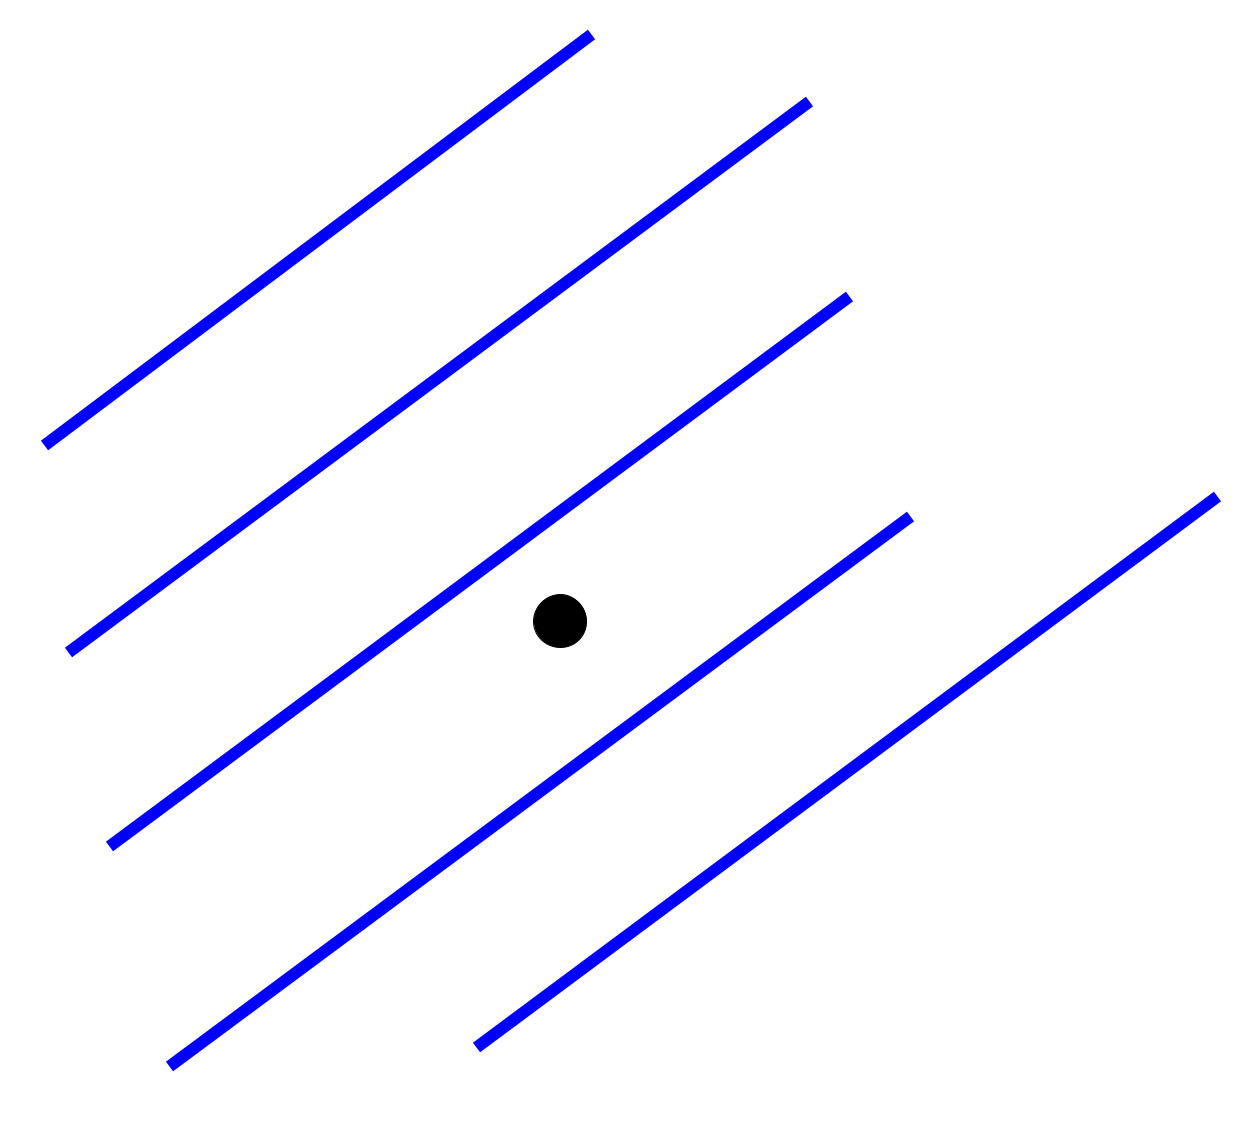
\includegraphics[width=.7\linewidth]{img/zonotopes/convexHullParallelLines1.png}
      \caption{A set of parallel lines and a random chosen point.}
      \label{im:convexHullParallelLines1}
    \end{minipage}\hfill
    \begin{minipage}{0.48\textwidth}
      \centering
      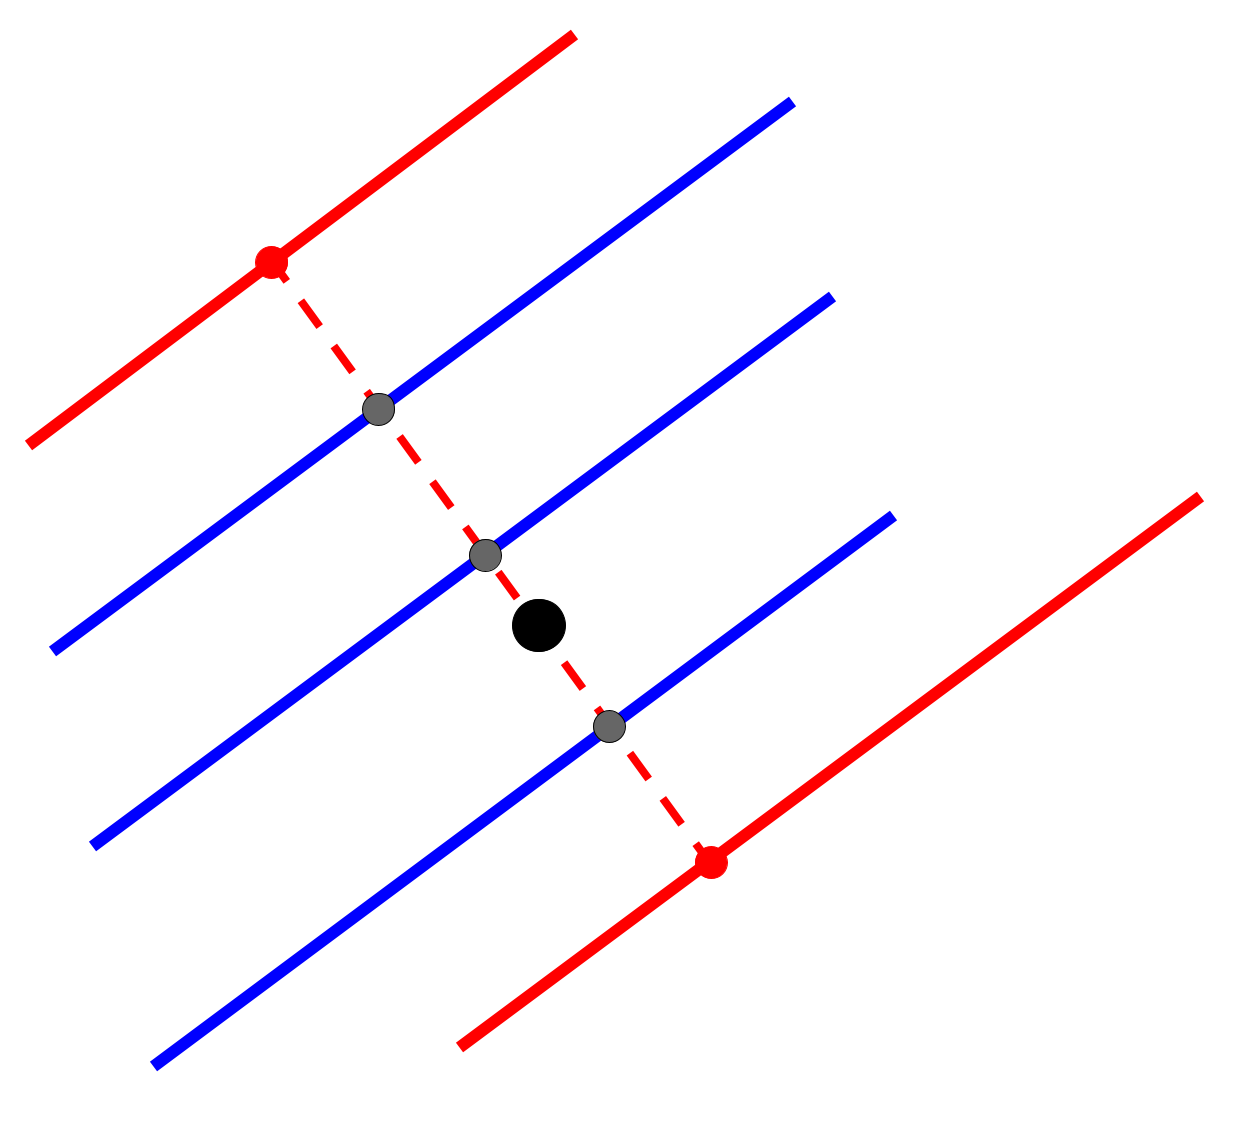
\includegraphics[width=.7\linewidth]{img/zonotopes/convexHullParallelLines2.png}
      \caption{In blue: the original set of parallel lines; in red: the convex hull of this set.}
      \label{im:convexHullParallelLines3}
    \end{minipage}
 \end{figure}

\begin{figure}[ht]
    \centering
    \begin{minipage}{.8\linewidth}
        \begin{algorithm}[H]
            \SetAlgoLined
            \KwData{$S = \{ L_1,\,\dots,\, L_k \}$ a set of parallel lines in $\mathbb{R}^n$}
            \KwResult{$S' := \text{conv}(S)$ the convex hull of $S$}
            $U\gets \emptyset$\;
            $S'\gets \emptyset$\;
            \ForEach{$L\in S$}{
                $p_L\gets \text{orthogonal projection of } \mathbf{0}_{\mathbb{R}^n} \text{ onto } L$\;
                $U \gets U\cup\{p_L\}$
            }
            \ForEach{$p_L\in$ \normalfont{conv}$(U)$}{
                $S' \gets S'\cup \{L\}$
            }
            \Return{$S'$}
            \caption{The convex hull of a set of parallel lines}
            \label{alg:convexHullParallelLines}
        \end{algorithm}
    \end{minipage}
\end{figure}


\subsubsection{The algorithm}
Constructing the 5D hypercube requires to duplicate the 4D hypercube and link each 4D-vertex to its duplicate version.
The process continues until the $m$th dimension is reached.

To enumerate vertices of a zonotope, a naive algorithm would enumerate all cube vertices then compute the convex hull on 
their projection. However, the HSM algorithm computes the $\mathcal{H}$-representation of a zonotope for a given set of generators, so 
a conversion between the $\mathcal{H}$ and $\mathcal{V}$-representation must be applied on the found solution.
Our proposed algorithm computes the edges of a zonotope, which are projection of the cube edges. Then, since a vertex can be found
at either side of an edge, the conversion to a $\mathcal{V}$-representation is fast.


\begin{figure}[ht]
    \centering
    \begin{minipage}{.6\linewidth}
        \begin{algorithm}[H]
            \SetAlgoLined
            \KwData{A matrix $N \in \mathbb{R}^{n\times m}$, a cube $C^m$}
            \KwResult{Edges of the zonotope $Z := NC^m$}
            $d\gets 2$\;
            $N_d\gets N[:,:d]$\;
            $Z_d\gets \emptyset$\;
            $E\gets \{\text{edges of the 2D cube}\}$ \;
            \While{$d < m$}{
                $N_d\gets N[:,:d+1]$\;
                $E_d\gets \text{duplicateAndLink}(E, d)$\;
                $Z_d \gets \text{projectEdges}(N_d, E_d)$\;
                
                $E \gets \emptyset$\;
                \ForEach{group of parallel edges $G\in Z_d$}{
                    $E \gets E \cup \text{hull}(G)$\;
                }
                
                $d\gets d+1$
            }
            \caption{Zonotope edge enumeration algorithm}
        \end{algorithm}

    \end{minipage}
\end{figure}


\subsection{Results and discussion}

\begin{table}[]
    \centering
    \begin{tabular}{|l|l|l|l|l|}
    \hline
    $(n,\,m)$ & Naive & HSM  & Edges & Edges (parallelized) \\ \hline
    (6,7)       & $0.019\pm0.001$  & $0.023\pm 0.002$ & $0.033\pm 0.002$ & $\mathbf{0.022\pm 0.010}$   \\ \hline
    (6,9)       & $0.159\pm 0.011$ & $\mathbf{0.024\pm 0.273}$ & $0.216\pm 0.016$ & $0.083\pm 0.024$   \\ \hline
    (7,8)       & $0.232\pm 0.025$ & $0.246\pm 0.022$ & $0.203\pm 0.014$ & $\mathbf{0.062\pm 0.008}$   \\ \hline
    (7,9)       & $0.933\pm 0.064$ & $1.216\pm 0.005$ & $0.754\pm 0.026$ & $\mathbf{0.203\pm 0.019}$   \\ \hline
    (8,8)       & $0.761\pm 0.091$ & $0.764\pm 0.078$ & $0.365\pm 0.019$ & $\mathbf{0.101\pm 0.012}$   \\ \hline
    (8,9)       & $6.054\pm 0.577$ & $6.516\pm 0.885$ & $2.375\pm 0.101$ & $\mathbf{0.636\pm 0.042}$   \\ \hline
    \end{tabular}
    \caption{Mean and standard deviation of time computation in seconds for $20$ random zonotopes generated per $(n,\,m)$ combination
    with $n$ is the dimension of the zonotope $Z$ and $m$ the dimension of $C^m$. A convertion to vertices is applied on the results of HSM and Edges and 
    taken into account in the time computation. All the tests have been computed using a Dell XPS Windows 11 computer using a 16-core Intel i9 processor.}
\end{table}


Our algorithm has several advantages compared to the naive and HSM algorithms: it is parallelizable (during the \textit{foreach} part) 
and it is by construction computationally faster than the naive algorithm and HSM as the hypercube considered grows.

It should be noticed that if $n\leq 6$, the naive algorithm or HSM stays the best option, with the unparallelized zonotope edge enumeration algorithm having
reasonnably close time computation to them ($< 0.001$ seconds). Also, the parallelized version does have overhead due to sending computations on multiple processor cores 
so it is not efficient for $n < 6$. 


Zontope representation has a major drawbacks: it does assume that all muscle tensions can be exerted at the 
While it may seem to be a strong hypothesis on the relationship between tensions, we will show in chapter ...
that for a sufficient number of considered tensions, this relationship naturally vanishes and can be represented
in a orthotopic-shapelike.

\section{Representation in musculoskeletal models with a large number of muscles}
\subsection{Zonotope and ellipsoid representations}
Feasible torque space noticed as an ellipsoid-like shape.
\begin{itemize}
    \item \cite{baillargeonExperimentallyQuantifyingFeasible2022} baillargeon 2022
    \item \cite{baillargeonOlderAgeAssociated2024a} baillargeon 2024
\end{itemize}
\subsection{Projection constant and ellipsoidal approximation of zonotopes}
\subsection{Results and discussion}

\section{Identification of a class of cable models producing the same torque capacities}
\subsection{Cable geometry and tension relationship}
\subsection{$\mathcal{Z}_{\tau}$-equivalent cable models}
\subsection{Identification algorithm}
\subsection{Results and discussion}
\section{Conclusion}